\chapter{Operace s gramatikami}
	
	Operace s~gramatikami můžeme obecně rozdělit na transformační (mění podobu gramatiky) a~parsovací (zpracovávají text). V~rámci parsovacích operací se snažíme o~nejefektivnější validaci vstupu za současného převodu do struktur vhodných pro další zpracování. Tyto struktury se mohou v závislosti na úrovni abstrakce a potřebě zasahovat do procesu zpracování měnit. Běžně používanou reprezentací je již zmiňovaný abstraktní syntaktický strom, kterým se budeme zabývat dále v práci. Další běžně známou reprezentací je Java bytecode, který je překládán až na cílové platformně při spuštění aplikace. \gls{gloss:GCC} například podporuje několik reprezentací: Register Transfer Language, \gls{gloss:LLVM}, Static single assignment form a další.
	
	Z~hlediska transformačních operací jde o~vytvoření nové, optimalizované gramatiky, která bude generovat stejný jazyk jako gramatika původní. To je případ i algoritmů pro převod gramatiky do \gls{gloss:CNF}. Tyto transformace jsou známé a~popsané. Transformace, které mění generující jazyk, jsou méně obvyklé, protože vyžadují širší kontext a náročnou intelektuální práci, kterou je téměř nemožno algoritmizovat. Tyto transformace dovolují změnit gramatiku do podoby, kterou je možno parsovat rychlejším parsovacím algoritmem. Pokud je generovaný jazyk podmnožinou (resp. nadmnožinou nebo kombinací) původního jazyka, musí se rozdíly zpracovat v~pozdějších fázích překladu.
	
	\section{Problémy transformací}
	
	Na druhou stranu i transformace, neměnící generovaný jazyk, mohou měnit syntaktickou strukturu. To je nežádoucí, protože v~rámci atributovaných gramatik (či jiného způsobů zpracování) předpokládáme strukturu definovanou naší gramatikou. Aplikováním transformací se gramatika (a tím i~syntaktická struktura) změní.
	
	\begin{figure}
	\begin{lstlisting}[escapeinside={(*}{*)}]
STATEMENT (* $\rightarrow$ *) if CONDITION STATEMENT STATEMENT
STATEMENT (* $\rightarrow$ *) (* \dots *)
CONDITION (* $\rightarrow$ *) (* \dots *)
	\end{lstlisting}
	\caption{Ukázka gramatiky představující \enquote{if statement}}
	\label{pic:ifStatementDemo}
	\end{figure}

	\begin{figure}
		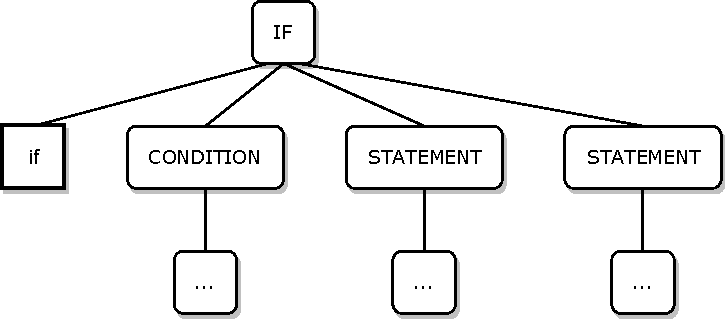
\includegraphics[width=0.45\textwidth]{img/DemoIfStatement}
		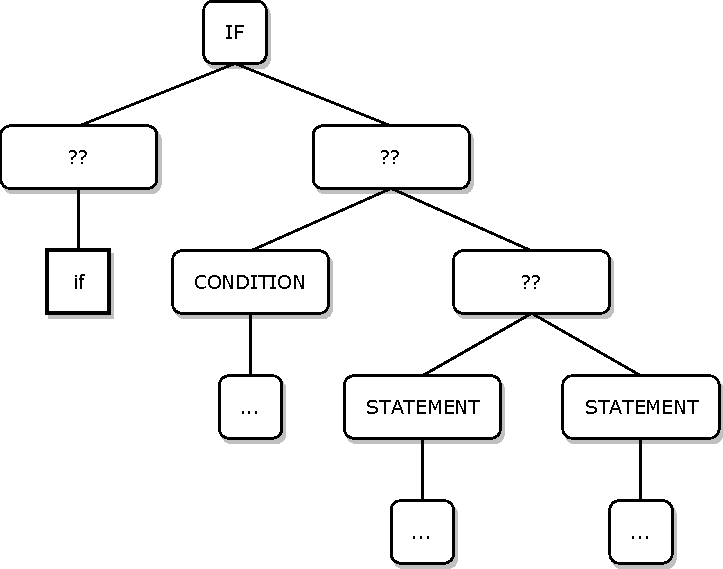
\includegraphics[width=0.45\textwidth]{img/DemoIfStatementWithTransformation}
		\captionof{figure}{Očekávaný a~reálný syntaktický strom pro \enquote{if statement}}
		\label{pic:ifStatemenAST}
	\end{figure}
	
	Pro představu budeme situaci demonstrovat na jednoduché gramatice (obrázek \ref{pic:ifStatementDemo}), převedené do \gls{gloss:CNF}.
	Po naparsování vstupu bychom očekávali výstup jako na obrázku \ref{pic:ifStatemenAST} vlevo. Ale vzhledem k~transformacím gramatiky bude výsledek odlišný (obrázek \ref{pic:ifStatemenAST} vpravo).
	
	To je z~hlediska sémantické analýzy komplikace, protože v~době tvorby gramatiky netušíme, jak bude gramatika transformovaná a to nám brání v~dodání sémantického významu pro modifikovaný \gls{gloss:AST}. Z~tohoto důvodu musí knihovna obsahovat i funkcionalitu ke zpětné rekonstrukci syntaktického stro\-mu podle původní netransformované gramatiky.
	
	\section{Převod do Chomského normální formy} 
	
	Práce dále popisuje všechny transformace i s~jejich pseudokódem. Po pseudokódu následuje popis zpětné transformace (pokud dává smysl), možné dopady na původní transformaci a popis změn v parsovacím procesu. Jednotlivé algoritmy, jejich popis a~pseudokód vychází z~materiálu \cite{Meduna:2014:FLC:2636678}.
	
	\subsection{Odstranění negenerujících symbolů}
	
	Vhodným příkladem může být gramatika pouze s~jediným pravidlem $S \rightarrow x S$. Všechny větné formy generované takovou gramatikou obsahují neterminál, generovaný jazyk je tedy prázdný.
	
	Odstranění negenerujících symbolů nemění syntaxi gramatiky (protože odstraněná část se nemůže vyskytnout v~žádné větné formě generujícího slova), ale zjednodušuje ji a tím snižuje časové a paměťové nároky na algoritmy, které dále s~gramatikou pracují.
	
	Algoritmus pro odstranění negenerujících symbolů si drží množinu symbolů, které tvoří libovolnou větu. Na počátku jsou v~této množině pouze terminály. Algoritmus poté hledá pravidla, které se přepíší na již generující symboly. Pokud takové pravidlo nalezne, přidá symbol na levé straně pravidla mezi generující symboly a postup opakuje.
	
	Algoritmus končí ve chvíli, kdy jsou zpracována všechna pravidla a žádný další generující symbol není přidán. Algoritmus poté z~gramatiky vymaže všechny negenerující symboly a s~nimi i všechna pravidla, která tyto symboly obsahují. Za předpokladu, že je gramatika konečná, algoritmus skončí po konečném počtu kroků. Pseudokód algoritmu je kód \ref{alg:removeNongeneratingSymbols}.
	
	\begin{listing}[h]
		\begin{minted}[tabsize=3]{text}
odstranění_negenerujících_symbolů(gramatika):
	generující = gramatika.terminály
	opakuj dokud se generující množina nezměnila:
		pro každé pravidlo v gramatice:
			jsou-li všechny symboly pravé strany generující:
				generující.přidej(pravá strana pravidla)

	odstranit = gramatika.nonterminály - generující
	gramatika.odstran(odstranit)
		\end{minted}
		\caption{Pseudokód algoritmu odstraňující negenerující symboly}
		\label{alg:removeNongeneratingSymbols}
	\end{listing}
	
	Pro algoritmus není nutné implementovat zpětnou transformaci, protože nemění syntaktickou strukturu gramatiky, ale pouze gramatiku optimalizuje.
	
	Speciální situace nastává ve chvíli, kdy algoritmus označí počáteční symbol gramatiky jako negenerující. V takovém případě gramatika generuje prázdný jazyk a v dalších algoritmech nemusíme pokračovat.
	
	\subsection{Odstranění nedostupných symbolů}
	Odstranění nedostupných symbolů je, stejně jako odstranění negerujících symbolů, pouze optimalizační technika, která snižuje velikost gramatiky a~tím i~časové a paměťové nároky  dalších algoritmů, které s~gramatikou pracují.
	
	Algoritmus pro odstranění nedostupných symbolů je velmi podobný algoritmu pro odstranění negenerujících symbolů, pouze prochází gramatiku v~opačném směru. Algoritmus si drží množinu dostupných symbolů, do které na počátku vloží počáteční symbol. Poté prochází pravidla a~pro ta, jejichž levá strana je obsažena v~množině, vloží do množiny dostupných symbolů také všechny symboly pravé strany. Pseudokód je kód \ref{alg:removeNonreachableSymbols}.
	
	\begin{listing}[h]
		\begin{minted}[tabsize=3, breaklines]{text}
odstranění_nedostupných_symbolů(gramatika):
	dostupné = gramatika.počáteční_symbol
	opakuj dokud se množina dostupných symbolů nezměnila:
		pro každé pravidlo v gramatice:
			je-li levá strana pravidla v dostupné:
				dostupné.přidej(pravá strana)

	odstranit = gramatika.nonterminály
	            + gramatika.terminály 
	            - dostupné
	gramatika.odstran(odstranit)
		\end{minted}
		\caption{Pseudokód algoritmu odstraňující nedostupné symboly}
		\label{alg:removeNonreachableSymbols}
	\end{listing}
	
	Na rozdíl od algoritmu pro odstranění negenerujících symbolů mohou být během běhu algoritmu odstraněny i terminály. Terminály mohou být odstraněny všechny, a to ve chvíli, kdy gramatika generuje pouze \Eps.
	
	\subsection{Odstranění \EpsS pravidel}
	
	Bezkontextové gramatiky mají obecný tvar pravidla $X\rightarrow\TermNontermIter$. V~takové gramatice lze (na rozdíl od gramatik regulárních a kontextových) derivovat libovolný symbol na \EpsS (obsahuje-li gramatika příslušná pravidla). To by komplikovalo parsovací proces, protože by byla gramatika zkracující.
	
	Cílem algoritmu je transformovat gramatiku s~\Eps~pravidly na gramatiku bez \Eps~pravidel a~tím ji udělat nezkracující.
	
	Algoritmus nejprve nalezne všechny neterminály, které jsou přímo nebo nepřímo derivovatelné na \Eps. Postup je velmi podobný jako u algoritmu pro odstranění negenerujících symbolů, pouze s~tím rozdílem, že na počátku algoritmu vložíme do generujících symbolů pouze \Eps. Pseudokód je kód \ref{alg:searchEpsilonGenerating}.
	
	\begin{listing}[h]
		\begin{minted}[tabsize=3]{text}
nalezení_neterminálů_přepisovatelných_na_epsilon(gramatika):
	generujici = vytvoř množinu
	opakuj dokud se generujici množina nezměnila:
		pro každé pravidlo v gramatice:
			jsou-li všechny symboly pravé strany přepisovatelné:
				generujici.přidej(pravá strana)

	vrať přepisovatelné
		\end{minted}
		\caption{Pseudokód algoritmu hledající neterminály generující \Eps}
		\label{alg:searchEpsilonGenerating}
	\end{listing}
	
	Poté algoritmus projde všechna pravidla. Pravidla, která se přímo přepisují na \Eps~jsou z~gramatiky vyloučena. Touto operací dojde k modifikaci gramatiky a tím i ke změně generujícího jazyka. To je pro další práci nepřípustné, protože jako výstup požadujeme gramatiku generující stejný jazyk.
	
	\paragraph{Vyloučení pravidla}
	je proces, který z gramatiky odebere pravidlo bez toho, aniž by byl změněn generující jazyk. Nechť \GrammarDef\space je bezkontextová gramatika a v~ní pravidlo $\rho=A\rightarrow\alpha$, které vyloučíme. Jestliže ke všem pravidlům $X\rightarrow\gamma A \delta$ přidáme pravidlo $X\rightarrow\gamma\alpha\delta$, potom se generovaný jazyk nezmění.
	
	\vspace{1em}
	
	Věta nám říká, že nahradíme-li ve všech pravidlech neterminál, který je na levé straně vyloučeného pravidla, pravou stranou vyloučeného pravidla, poté gramatika popisuje stejný jazyk. Pseudokód je kód \ref{alg:removeRule}.
	
	\begin{listing}[h]
		\begin{minted}[tabsize=3]{text}
odstraň_pravidlo(gramatika, pravidlo):
	gramatika.odstraň(pravidlo)
	pro každé pravidlo p_1 v gramatice:
		pro každý symbol v p_1.pravá_strana:
			jestliže symbol = pravidlo.levá_strana:
				nové = nahraď symbol pravou stranou pravidla
				gramatika.přidej(nové)
		\end{minted}
		\caption{Pseudokód algoritmu odstraňující pravidlo}
		\label{alg:removeRule}
	\end{listing}
	
	V našem případě odstraňujeme pouze \EpsS pravidla (pravidla typu $X\rightarrow\varepsilon$). Během odstranění se modifikovaná pravidla zkracují (například z~pravidel $\left\{\right.A\rightarrow B,$ $B\rightarrow\varepsilon\left.\right\}$ vznikne $\left\{A\rightarrow B, A\rightarrow\varepsilon\right\}$), může se tedy stát, že vznikne nové \EpsS pravidlo. Algoritmus proto opakuje postup tak dlouho, dokud v~gramatice existují \EpsS pravidla. Pseudokód je kód \ref{alg:removeEpsilonRules}.
	
	\begin{listing}[h]
		\begin{minted}[tabsize=3]{text}
odstranění_epsilon_pravidel(gramatika):
	dokud v gramatice existují epsilon pravidla:
		pravidlo = najdi_epsilon_pravidlo(gramatika)
		odstraň_pravidlo(pravidlo)
		\end{minted}
		\caption{Pseudokód algoritmu odstraňující \EpsS pravidla}
		\label{alg:removeEpsilonRules}
	\end{listing}
	
	Tato verze algoritmu má velkou časovou složitost, protože opakovaně prochází všechna pravidla v~gramatice. Algoritmus lze optimalizovat použitím fronty a množiny symbolů derivovatelných na \Eps. Algoritmus poté prochází každé pravidlo pouze jednou.
	
	%			\begin{listing}[h]
	%				\begin{minted}[tabsize=3]{text}
	%odstranění_epsilon_pravidel(gramatika):
	%	přepisovatelné = nalezení_neterminálů_na_epsilon(gramatika)
	%	pravidla = vytvoř_frontu(gramatika.pravidla)
	%	dokud fronta pravidla není prázdná:
	%		pravidlo = další_prvek_ve_frontě(pravidla)
	%		pokud se praidlo.pravá_strana rovná epsilon:
	%			gramatika.odstraň(pravidlo)
	%			opakuj
	%		pro každý symbol v pravidlo.pravá_strana:
	%			pokud je symbol přepisovatelný:
	%				nové = vytvoř_pravidlo_bez_symbolu(pravidlo, symbol)
	%				gramatika.přidej(nové)
	%				pravidla.přidej(nové)
	%			\end{minted}
	%			\caption{Pseudokód optimalizovaného algoritmu odstraňující \EpsS pravidla}
	%		\end{listing}		
	
	Pro algoritmus odstranění \EpsS symbolů již potřebujeme algoritmus zpětné transformace syntaktického stromu. Při transformaci se pro nově vytvořená pravidla (tedy pravidla s odstraněným \EpsS symbolem) uloží pravidlo, ze kterého nové pravidlo vzniklo, a symbol, který byl přepsán na \Eps. Na základě těchto informací je algoritmus schopen určit originální pravidlo a syntaktický strom transformovat tak, aby odpovídal originální gramatice.
	
	\subsection{Odstranění jednoduchých pravidel}
	
	Algoritmus pro odstranění jednoduchých pravidel je podobný tomu pro odstranění \Eps~pravidel. Algoritmus ve své nejjednodušší implementaci vylučuje jednoduchá pravidla až do doby, pokud v~gramatice ještě nějaká existují. Optimalizovaná verze algoritmu má několik kroků, ale má nižší časové a~paměťové nároky. Jedná se o~pseudokód \ref{alg:removeUnitRules}.
	
	\begin{enumerate}
		\item
		Algoritmus vytvoří tranzitivní uzávěr jednoduchých pravidel.
		\item
		Algoritmus odstraní z~gramatiky všechna jednoduchá pravidla.
		\item
		Algoritmus prochází zbylá pravidla a~vybere ta, pro která v~gramatice existuje neterminál derivovatelný jednoduchými pravidly na levou stranu procházeného pravidla.\par
		Dále předpokládejme, že mluvíme o~obecném pravidlu $\Rule{X}{Ab}$ a~neterminálu $Z$ takovém, že existuje derivce $Z \Rightarrow X$ za použití pouze jednoduchých pravidel.
		\item
		Algoritmus vytvoří nové pravidlo. Na levé straně pravidla bude procházený neterminál a~na pravé straně pravá strana procházeného pravidla. Algoritmus tedy vytvoří pravidlo $\Rule{Z}{Ab}$.
		\item
		Vytvořené pravidlo přidá do gramatiky
	\end{enumerate}
	
	\begin{listing}
		\begin{minted}[tabsize=3]{text}
odstranění_jednoduchých_pravidel(gramatika):
	uzávěr = tranzitivní uzávěr jendoduchých pravidel
	pro každé pravidlo p_1 gramatiky:
		jestliže je p_1 jednoduché:
			gramatika.odstraň(p_1)
			pokračuj s dalším pravidlem
		pro každý neterminál n_1:
			pokud lze derivovat n_1 na p_1.levá_strana
				nové = pravidlo(n_1, p_1.pravá_strana)
				gramatika.přidej(nové)
		\end{minted}
		\caption{Pseudokód algoritmu odstraňující jednoduchá pravidla}
		\label{alg:removeUnitRules}
	\end{listing}
	
	Při algoritmu zpětné transformace je nutné pro nově vytvořené pravidlo uložit sérii jednoduchých pravidel, na základě kterých bylo pravidlo vytvořeno. Algoritmus dokáže podle této informace určit, která jednoduchá pravidla byla použita při odstranění, a z~toho vyvodit správnou podobu syntaktického stromu.
	
	\subsection{Převod na Chomského normální tvar}
	
	Připomeňme, že \gls{gloss:CNF} vyžaduje pravidla ve třech podobách:
	\begin{itemize}
		\item $A \rightarrow B C$,
		\item $A \rightarrow a$,
		\item $S \rightarrow \varepsilon$.
	\end{itemize}
	Po dokončení předchozích algoritmů máme jistotu, že se v gramatice nevykytuje pravidlo derivující se na \EpsS nebo jednoduchá pravidlo. Transformace do \gls{gloss:CNF} již probíhá jednoduše podle následujícího postupu.
	\begin{itemize}
		\item Pravidla vyhovující CNF ponecháme.
		\item Pravidla tvaru $A\rightarrow\alpha a \beta$ nahradíme pravidly $\left\{A\rightarrow\alpha a' \beta,\allowbreak a'\rightarrow a\right\}$ kde $a$~je terminál a~$a'$ je nový neterminál, dosud v~gramatice nepoužitý.
		\item Pravidla delší než dva neterminály rozdělíme vytvořením nových neterminálů a pravidel. Pravidlo $$A\rightarrow B_1 B_2 \cdots B_k$$ 
		rozdělíme na 
		\begin{flalign*}
				\left\{\right.
				&
				A\rightarrow B_1 \left<B_2\cdots B_k\right>, 
				\left<B_2\cdots B_k\right>\rightarrow B_2 \left< B_3\cdots B_k\right>, 
				\cdots, 
				&&\\
				&
				\left<B_{k-2}B_{k-1}B_k\right>\rightarrow B_{k-2} \left<B_{k-1}B_k\right>,
				\left<B_{k-1}B_k\right>\rightarrow B_{k-1} B_k
				\left.\right\} 
				&&
		\end{flalign*}
		kde $\left<\cdots\right>$ jsou nové neterminály, dosud v~gramatice nepoužité.
	\end{itemize}
	
	Pro algoritmus zpětné rekonstrukce nám postačí ukládat, o který ze dvou bodů výše se jedná, současně s pravidlem, ze kterého bylo nové pravidlo vytvořeno. Poté stačí uzel v syntaktickém stromu nahradit jeho správným ekvivalentem. V případě druhého bodu nahradíme uzel samotným terminálem, ve třetím případě (rozdělení pravidla) získáme zbytek neterminálů jako potomky pravého potomka.
	
	\section{Cocke-Younger-Kasami algoritmus}
	
	Cocke-Younger-Kasami algoritmus \cite{Younger1967} (nebo též \gls{gloss:CYK}) je jeden z parsovacích algoritmů pro bezkontextové gramatiky. Na rozdíl od zmíněných parsovacích algoritmů (jako LL a LR algoritmy) je schopen zpracovat libovolnou bezkontextovou gramatiku včetně nejednoznačné. Algoritmus je v takovém případě nedeterministický, ale konečný a~\gls{gloss:CYK} je schopen vstupní slovo naparsovat. Jedná se o~hlavní vlastnost, kvůli které byl algoritmus pro tuto práci vybrán.
	
	Jeho nevýhodou je zvýšená časová a paměťová náročnost. Časová složitost je v~nejhorším případě $\mathcal{O}(n^3 \cdot |G|)$, kde $|G|$ je počet pravidel v gramatice a $n$ je délka vstupního slova. Paměťová složitost je v nejhorším případě $\mathcal{O}(n^2 \cdot |G|)$. Další nevýhodou je neschopnost odhalovat chyby. Algoritmy pracující se slovem lineárně jsou schopny označit konkrétní symbol nevyhovující definici gramatiky. \gls{gloss:CYK} algoritmus odhalí nevalidní vstup, ale vzhledem k~jeho konstrukci není schopen určit místo, na kterém k~chybě došlo.
	
	\gls{gloss:CYK} algoritmus je založen na dynamickém programování. Algoritmus nej\-dří\-ve najde neterminály, které se přímo derivují na terminály vstupního slova (tj. použije všechny možné $X\rightarrow a$ pravidla). Algoritmus dále hledá všechny neterminály, které se derivují na podslova délky $2,3,\cdots,n$ obsažené ve vstupním slovu. Přitom využívá faktu, že slovo délky $k$ jsou dvě slova délek $(k-1,1),(k-2,2),\cdots,(2,k-2),(1,k-1)$. Pokud se v neterminálech, které generující celé vstupní slovo, vykytuje startovací symbol, potom je vstup úspěšně naparsován a algoritmus může vytvořit syntaktický strom.
	
	Běh algoritmu budeme dále v~textu demonstrovat tabulkou. První řádek tabulky budou neterminály generující vstupní slovo (tedy slovo délky $n$), druhý řádek část slova délky $n-1$, třetí řádek část slova délky $n-2$ atd. Na posledním řádku tabulky budou neterminály, které se přímo derivují na symboly vstupního slova.
	
	Proces budeme demonstrovat na gramatice \Grammar{a,b}{S,A,B,C}{S}{
		S \rightarrow A B,
		S \rightarrow B C,
		A \rightarrow B A,	
		A \rightarrow a,
		B \rightarrow C C,
		B \rightarrow b,
		C \rightarrow A B,
		C \rightarrow a,
	} \\ a slovu $w=aaba$.
	
	Algoritmus nejdříve zjistí, které neterminály se přímo derivují na symboly slova (například neterminály $A$ a $C$ se derivují na $a$). Ve druhém kroku tvoří slovo délky 2. Například neterminál $B\Rightarrow CC\Rightarrow aa$. Ve třetím kroku tvoří slova délky 3, tzn. kombinace slova délky 1 a slova délky 2 nebo slovo délky 2 a~slovo délky 1. Pro neterminál $B$ se použilo pravidlo $B\rightarrow CC$, kde první neterminál $C$ je~na třetím řádku a druhém sloupci (slovo délky 2) a druhý neterminál $C$ na čtvrtém a řádku čtverém sloupci (slovo délky 1). Neterminál $B$ skutečně generuje slovo délky 3, tedy $B\Rightarrow CC \Rightarrow ABC \Rightarrow aba$. V posledním kroku algoritmus detekuje, které neterminály lze derivovat do vstupního slova. V prvním žádku se vykytuje počáteční symbol $S$, a tedy je slovo generováno pravidly $S \Rightarrow AB \Rightarrow ACC \Rightarrow AABC \Rightarrow aaba$.
	
	\begin{figure}
		\centering
		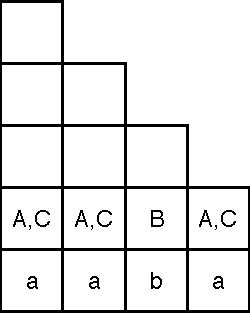
\includegraphics[width=0.22\textwidth]{img/CYKDemo1STEP1}
		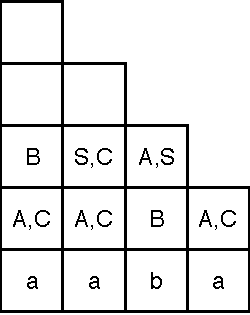
\includegraphics[width=0.22\textwidth]{img/CYKDemo1STEP2}
		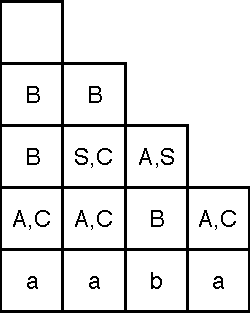
\includegraphics[width=0.22\textwidth]{img/CYKDemo1STEP3}
		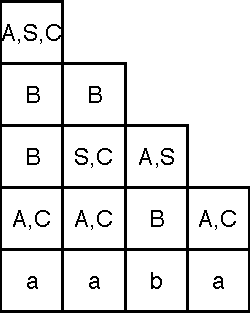
\includegraphics[width=0.22\textwidth]{img/CYKDemo1STEP4}
		\caption{Kroky \gls{gloss:CYK} algoritmu}
		\label{pic:cykSteps}
	\end{figure}
	
	Kód \ref{alg:cyk} poté slouží jako pseudokód \gls{gloss:CYK} algoritmu.
	
	\begin{listing}
		\begin{minted}[tabsize=3,escapeinside={(*}{*)}]{text}
pozice(řádek, sloupec):
	kombinace = vytvoř množinu
	počet_kombinací = délka slova - řádek
	pro v jdoucí do počet_kombinací:
		b_1 = bod(řádek + v + 1, sloupec)
		b_2 = bod(řádek + počet_kombinací - v, 
		          sloupec + počet_kombinací - v)
		kombinace.přidej((b_1, b_2))
	vrať kombinace
	
cyk(gramatika, slovo):
	pole = vytvoř dvojrozměrné pole veliksoti délky slova
	pro každý symbol slova:
		pravidla = najdi pravidla derivující se na symbol
		pole[délka slova][index] = pravidla.levá_strana	
	pro každý řádek i:
		pro každý sloupec j:
			pro každý prvek (b_1, b_2) v pozice(i, j):
				první_s = pole[b_1.x][b_1.y]
				druhý_s = pole[b_2.x][b_2.y]		
				pro každé pravidlo p_1:
					pokud p_1.pravá_strana = (první_s, druhý_s)
						pole[i][j] += p_1.levá_strana
	jestliže je gramatika.počáteční_symbol v pole[0][0]:
		úspěch
	jinak:
		neúspěch
		\end{minted}
		\caption{Pseudokód \gls{gloss:CYK} algoritmu}
		\label{alg:cyk}
	\end{listing}
	
	Pro samotnou konstrukci syntaktického stromu je potřeba algoritmus upravit. \gls{gloss:CYK} algoritmus během svého běhu nebude do tabulky ukládat neterminály, které se derivují na slovo, ale uloží si použité pravidlo a pozice symbolů pravé strany pravidla. Díky těmto informacím může algoritmus po úspěšném parsování sestavit syntaktický strom bez dodatečného procházení gramatiky nebo vstupního slova.